\chapter{Narrow Band Transmission}
\label{chap:res_450}
First, a system transmitting at only a quarter of the maximal symbol rate
was build and analyzed to show some basic properties of the system and
to show what the best achievable \gls{EVM} values are. \\

As receiver architecture, the Quadrature Intermediate Frequency Sub-Nyquist
Sampling Receiver as described in \secref{sec:rx_2} is used with the difference
that the signal bandwidth is only $B = 450 MHz$. All the other properties are listed
in \tblref{tab:res_450}. \\

\begin{table}[h]
  \centering
  \begin{tabular}{|l|r@{}l@{~}l|}
    \hline
    $f_{\text{TX IF}}$ & 2&.9&GHz \\ \hline
    $f_{\text{TX LO}}$ & 57&.5&GHz \\ \hline
    $f_{\text{RX LO}}$ & 58&.2&GHz \\ \hline
    $f_{\text{RX IF}}$ & 2&.2&GHz \\ \hline
    $f_c$            & 60&.4&GHz \\ \hline
    Signal Bandwidth B & 0&.45&GHz \\ \hline
    Sample Rate $f_s$ & 1&.8&GHz \\ \hline
  \end{tabular}
  \caption{Properties of Narrow Band Transmission System}
  \label{tab:res_450}
\end{table}

\section{Measurement Setup and RF System Analysis}
\label{sec:res_450_setup}

A block diagram providing an overview of the test setup,
used for all following measurements, can be found in \figref{fig:res_450_bd}. \\

\begin{figure}[p]
  \centering
  \includegraphics[width=\textwidth]{figures/res_450_setup}
  \caption{Block Diagram of the Narrow Band Transmission Setup}
  \label{fig:res_450_bd}
\end{figure}

\begin{figure}[p]
  \centering
  \includegraphics[width=\textwidth]{pictures/res_450_setup}
  \caption{Picture of the Narrow Band Transmission Setup}
  \label{fig:res_450_pic}
\end{figure}

\subsection{Matlab}
The Matlab script was configured such that it generates the transmit signal,
programs the \gls{AWG}, reads the data acquired by the \gls{FPGA},
runs the receiver code and finally generates reports and figures. \\

All measurements in this chapter are based on two different transmit
configurations.
One used \gls{QAM}-4 and the other one \gls{QAM}-256 to
modulate the data. The important properties can be found in
\tblref{tab:res_450_cnf}.
The configuration file used for these tests can be found in
\appref{app:res_450_cnf}. \\

\begin{table}[h]
  \centering
  \begin{tabular}{|c|c|c|}
    \hline
    Modulation of Data Fields & \gls{QAM}-4 & \gls{QAM}-256 \\ \hline
    Modulation of Estimation Fields & \mc{2}{\gls{BPSK}} \\ \hline
    Length of \gls{FES} field & \mc{2}{256 symbols} \\ \hline
    Length of \gls{CES} field & \mc{2}{1152 symbols} \\ \hline
    Length of \gls{PES} field & \mc{2}{32 symbols} \\ \hline
    Length of Data Block & \mc{2}{147 symbols} \\ \hline
    Length of Data Field & 115 symbols, 230 bits & 115 symbols, 920 bits \\ \hline
  \end{tabular}
  \caption{Properties of the Matlab Configuration used in the
    Narrow Band Transmission Setup (all lengths are in symbols)}
  \label{tab:res_450_cnf}
\end{table}

\subsection{\gls{AWG}}
The \gls{AWG} was configured to output the \gls{TX} \gls{IF} signal $i[k]$,
the sample clock for the \gls{ADC} as well as synchronization pulses to trigger
the \gls{FPGA} and oscilloscope. It's configuration and port assignment
are shown in \tblref{tab:res_450_awg}.

It was noticed, that the used \gls{AWG} has some cross talk from
channel 1 marker 1 output to the channel 1 analog output. Therefor the
\gls{ADC} clock should always be on marker 2 and not on marker 1.
For synchronization pulses, this is not an issue, since they were always
configured to give a 100 cycle wide positive pulse $> 100 \; \text{ns}$ before
the signal starts. \\

\begin{table}[h]
  \centering
  \begin{tabular}{|l|l|}
    \hline
    Sampling Rate & 10.8 GS/s \\ \hline
    Clock Source & Externals 10 MHz \\ \hline
    Analog Amplitude & 1 $\text{V}_{\text{pp}}$ \\ \hline
    Marker Amplitude CH1 Marker 1/2 & 0, 0.7 V \\ \hline
    Marker Amplitude CH2 Marker 1/2 & 0, 1.4 V \\ \hline
    \gls{DAC} resolution & 8 bit \\ \hline
    CH 1 & $i[k]$ \\ \hline
    CH 2 & $\mathcal{H}\{i[k]\}$ \\ \hline
    CH 1 Marker 1 & 0 \\ \hline
    CH 1 Marker 2 & 1.8 GHz \gls{ADC} sample clock \\ \hline
    CH 2 Marker 1 / 2 & Sync pulse before frame starts \\ \hline
  \end{tabular}
  \caption{Configuration and Port Assignment of \gls{AWG}}
  \label{tab:res_450_awg}
\end{table}

An oscilloscope plot (see \secref{sec:comp_osci}) of the generated
\gls{TX} \gls{IF} signal and it's \gls{FFT} can be found in
\figref{fig:res_450_awg_analog}.
The \gls{ADC} clock signal and the sync pulse are shown
in \figref{fig:res_450_awg_digital}. \\

\begin{figure}[p]
  \centering
  \includegraphics[width=\textwidth]{figures/osci/res_450_awg_analog}
  \caption{\gls{TX} \gls{IF} signal generated by the \gls{AWG}}
  \label{fig:res_450_awg_analog}
\end{figure}

\begin{figure}[p]
  \centering
  \includegraphics[width=\textwidth]{figures/osci/res_450_awg_digital}
  \caption{\gls{ADC} clock signal and sync pulse generated by the \gls{AWG}}
  \label{fig:res_450_awg_digital}
\end{figure}

\subsection{RF parts}
The two analog channels generated by the \gls{AWG} have a total signal
power of -9.28 dBm each \eqref{eq:res_450_awg_pwr}. These signals were
than attenuated by 20 dB to be below the 1 dB output compression point of 10 dBm
of the 60 GHz converters even at full gain of 40 dB. \\

\begin{align}
  10 \cdot \log_{10}\left(
  10^{-25.812 \;\text{dBm} / 10} \cdot
  \frac{450 \;\text{MHz}}{10 \;\text{MHz}}
  \right) \approx -9.28 \;\;\text{dBm}
  \label{eq:res_450_awg_pwr}
\end{align}

The same 60 GHz converter was used for transmission and reception and
configured as shown in \tblref{tab:res_450_sivers} (configuration script
see \appref{app:res_450_cnf}).
A 10 MHz reference clock was fed from the \gls{AWG}.
An aluminum plate in a distance of about 15 cm was used as a reflector. \\

\begin{table}[h]
  \centering
  \begin{tabular}{|l|l|}
    \hline
    Reference Clock & external \\ \hline
    TX Oscillator Frequency & 57.5 GHz (0x038170) \\ \hline
    RX Oscillator Frequency & 58.2 GHz (0x038D60) \\ \hline
    TX Power & 0x80 \\ \hline
  \end{tabular}
  \caption{Configuration Parameters of 60 GHz Converter}
  \label{tab:res_450_sivers}
\end{table}

Both channels on the \gls{RX} side of the converter first connect to a
\gls{MC} BHP-1000+ high-pass filter. As we can see in \figref{fig:res_450_rx_if},
the \gls{TX} \gls{LO} leakage is attenuated by about 35 dB. Also the \gls{TX}
\gls{LSBand} signal (centered around 3.6 GHz) is about 17 dB weaker than
the desired \gls{TX} \gls{USBand} signal. This is due to the transmitter's
image rejection and the fact that the \gls{LSBand} signal is outside the
\gls{RF} specification of the converter. \\

\begin{figure}[p]
  \centering
  \includegraphics[width=\textwidth]{figures/osci/res_450_rx_if}
  \caption{Received \gls{IF} Signal before (left) and after (right) High-Pass Filter}
  \label{fig:res_450_rx_if}
\end{figure}

Next the signal is amplified by 12 dB to drive the \gls{ADC} input to about 70\%
as shown in \figref{fig:res_450_rx_amp}. \\

\begin{figure}[p]
  \centering
  \includegraphics[width=\textwidth]{figures/osci/res_450_rx_amp}
  \caption{Received \gls{IF} Signal before (left) and after (right) the Amplifier}
  \label{fig:res_450_rx_amp}
\end{figure}

Finally the signal is converted to a differential signal using a ADC-WB-BB Balun
(\secref{sec:comp_balun}), passes a \gls{DC} block (\secref{sec:comp_dc_block})
and is digitized by the \gls{ADC}. \\

The channel filter shown in \figref{fig:rx_2_bd} is therefor build using
the BHP-1000+ high-pass filter and the \gls{ADC} analog input bandwidth which
cuts of at about 2.8 GHz. \\

\section{Channel Characterization}
\subsection{Channel impulse response}
\label{sec:res_450_h}
First we should have a short look at the channel response of the simple
reflector. The estimated channel response using the Golay estimator and a
1152 long \gls{CES} field is shown in \figref{fig:res_450_qam4_h}.
As we can see, there is one very distinctive peak confirming one single,
more or less flat, reflector. \\

\begin{figure}[p]
  \centering
  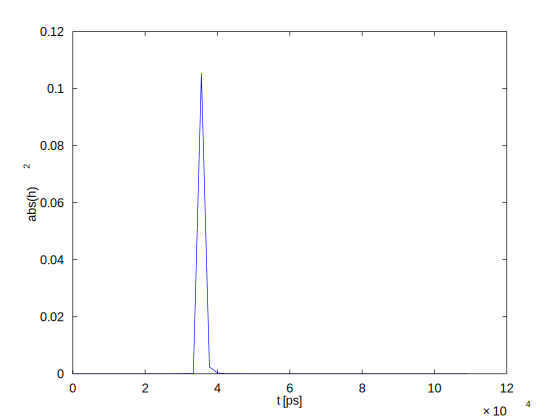
\includegraphics[width=0.8\textwidth]{figures/matlab/res_450_qam4_h}
  \caption{One realization of a Measured Channel Impulse Response in Time Domain
    with Narrow Band \gls{QAM}-4 Transmission Setup}
  \label{fig:res_450_qam4_h}
\end{figure}

\section{Error Vector Magnitude Definitions}
In this report, two different calculation schemes for the \acrfull{EVM}
are used.

\subsubsection{\acrfull{DEVM}}
The \gls{DEVM} uses the classical definition of the \gls{EVM}
and compares the received symbol to the their ideal position.
It is calculated as stated in \eqref{eq:devm} \cite{razavi2011rf}.

\begin{align}
  \text{EVM}_\text{D} &= \frac{1}{P_{\text{avg}}} \cdot \frac{1}{N}
  \sum_{j=0}^{N-1} |i_j - s_j|^2
  \label{eq:devm} \\
  \text{EVM}_\text{D}\text{dB} &= 10 \cdot \log_{10} (\text{EVM}_\text{D})
\end{align}

Where $N$ is the total number of symbols, $s_j$ the complex value of the
received symbol $j$ and $i_j$ the ideal position of the symbol. \\

\subsubsection{\acrfull{REVM}}
During the implementation phase and to show the improvements due to correction
algorithms, a second definition for the \gls{EVM} was used and
is called \gls{DEVM} in this report. This figure of merit is not influenced,
by deterministic errors due to a constant affine transformation of the
received symbols in the complex plane. \\

The proposed \acrfull{REVM} builds one subset of the set of received points for
each available data symbol. The error vector $e_j$ is than calculated as the
difference of the received point and the mean of all received points of that
set. Therefor it does not matter, if all points corresponding to one sent symbol
are off. Instead we have a figure of merit telling, how far one sent symbol gets
spread. \\

To get only one number in the end, the mean value of all the \gls{REVM}
calculated for the different symbols is used. \\

The calculation of the \gls{REVM} should only be used, if enough points
of each data symbols are used to calculate the means values which are then
used to calculate the error vectors $e_j$. This is the case for the \gls{QAM}-4
signal, where we expect $1752 / 2^2 = 438$ points per received symbol and
data block.
It isn't for the \gls{QAM}-256 signal, where we expect $1752 / 2^8 \approx 6.84$
points per received symbol and data block.

\subsubsection{\gls{EVM} per Data Block}
Both \gls{EVM} values can be calculated for the whole frame or for each
data block separately $\text{EVM}_\text{D,b}$ respectively
$\text{EVM}_\text{R,b}$.

\section{Correction Performance}
Next the the performance of the channel correction and the
phase noise correction will be analyzed. \\


\begin{table}[h]
  \centering
  \begin{tabular}{|l|l|r@{}l|r@{}l|r@{}l|r@{}l|r@{}l|r@{}l|}
    \hline
    &
    & \mc{2}{}
    & \mc{2}{}
    & \mc{2}{$\min$}
    & \mc{2}{$\max$}
    & \mc{2}{$\min$}
    & \mc{2}{$\max$} \\
    QAM & corrected
    & \mc{2}{\gls{REVM}}
    & \mc{2}{\gls{DEVM}}
    & \mc{2}{$\text{EVM}_\text{R,b}$}
    & \mc{2}{$\text{EVM}_\text{R,b}$}
    & \mc{2}{$\text{EVM}_\text{D,b}$}
    & \mc{2}{$\text{EVM}_\text{D,b}$} \\ \hline
    4   & ch.                         & - 1&.73 &   1&.52 & -34&.38 & -29&.70 & -32&.03 &   4&.35 \\ \hline
    4   & ch., ph. noise              & -31&.61 & -23&.88 & -34&.38 & -29&.70 & -27&.72 & -21&.00 \\ \hline
    4   & ch., ph. noise, initial ph. & -31&.61 & -30&.29 & -34&.38 & -29&.70 & -32&.54 & -26&.49 \\ \hline
    8   & ch.                         & - 0&.18 &   3&.70 &    &    &    &    &    &    &    &    \\ \hline
    8   & ch., ph. noise              & -28&.97 & -20&.44 &    &    &    &    &    &    &    &    \\ \hline
    8   & ch., ph. noise, initial ph. & -28&.97 & -28&.20 &    &    &    &    &    &    &    &    \\ \hline
  \end{tabular}
  \caption{Influence of the correction algorithms on the \gls{EVM} values
    of the Narrow Band Transmission System}
  \label{tab:res_450_evm}
\end{table}

\subsection{Uncorrected Signal}
It was already shown in the last section, that the energy of one sent symbol
is spread across multiple received symbols. Therefor we expect a huge
\gls{ISI} in the uncorrected signal which is shown in
\figref{fig:res_450_cp_rx}. \\

\begin{figure}[p]
  \centering
  \begin{subfigure}{0.45\textwidth}
    \centering
    \includegraphics[width=\textwidth]{figures/matlab/res_450_qam4_cp_rx}
    \caption{\gls{QAM}-4}
    \label{fig:res_450_qam4_cp_rx}
  \end{subfigure}
  ~
  \begin{subfigure}{0.45\textwidth}
    \centering
    \includegraphics[width=\textwidth]{figures/matlab/res_450_qam256_cp_rx}
    \caption{\gls{QAM}-256}
    \label{fig:res_450_qam256_cp_rx}
  \end{subfigure}
  \caption{One Realization of Data received by the Narrow Band
    Transmission Setup before any Correction}
  \label{fig:res_450_cp_rx}
\end{figure}

\subsection{Frequency Offset Estimation and Correction}
There was no need for any frequency estimation and correction, since all the
oscillators were looked to the same 10 MHz reference clock generated
by the \gls{AWG}. \\

\section{Channel Estimation and Correction}
The result of the the Golay estimator and the channel correction
as described in \secref{sec:sys_ces} are shown in \figref{fig:res_450_cp_corr}.
The different data blocks were colored differently. \\

As we can see in \figref{fig:res_450_qam4_cp_corr}, the \gls{ISI} was
corrected nicely but the received symbols are still spread on a circle
due to phase noise. \\

\begin{figure}[p]
  \centering
  \begin{subfigure}{0.45\textwidth}
    \centering
    \includegraphics[width=\textwidth]{figures/matlab/res_450_qam4_cp_corr}
    \caption{\gls{QAM}-4}
    \label{fig:res_450_qam4_cp_corr}
  \end{subfigure}
  ~
  \begin{subfigure}{0.45\textwidth}
    \centering
    \includegraphics[width=\textwidth]{figures/matlab/res_450_qam256_cp_corr}
    \caption{\gls{QAM}-256}
    \label{fig:res_450_qam256_cp_corr}
  \end{subfigure}
  \caption{One Realization of Data received by the Narrow Band
    Transmission Setup after Channel Correction}
  \label{fig:res_450_cp_corr}
\end{figure}

\subsection{Phase Noise Correction}
\label{sec:res_450_phase}
The $\max \text{EVM}_\text{R,b} = 29.70 \;\text{dB}$ value for the
\gls{QAM}-4 case shows, that, when the phase noise can be fully compensated
for, a value of at least 29.70 dB should be reach for $\text{EVM}_\text{D}$. \\

\figref{fig:res_450_cp_corr_pcorr} shows the results, after phase noise
estimation and correction, as described in \secref{sec:sys_pes}, has been
activated. The phase noise estimations seem to nicely align all received
data blocks.
The $\text{EVM}_\text{D} = -23.88 \;\text{dB} \geq -29.70 \;\text{dB}$ is still
not where it should be though. This is due to the fact, that the whole
picture is slightly rotated. This is due to the phase not being
constant during the transmission of the relatively
long \gls{CES} field (1152 symbols) when transmitting at only 450 MS/s. \\

Therefor, an initial phase correction was implemented by measuring the phase
rotation between the middle of the \gls{CES} field an the first \gls{PES}
field. This was possible by choosing the \gls{PES} field to consist
of exactly these symbols of the \gls{CES} field. \\

The result can be seen in \figref{fig:res_450_cp_corr_pcorr_initial} and the
$\text{EVM}_\text{D} = -30.29 \;\text{dB}$ is finally only 1.32 dB worse than
$\text{EVM}_\text{R} = -31.61 \;\text{dB}$ which shows that the correction
works. \\

The phase estimations can also be used to produce a plot showing how the
phase noise affects the absolute phase over time
(see \figref{fig:res_450_qam4_phase_est}). \\

\figref{fig:res_450_qam4_evm} shows nicely, that the \gls{DEVM}
soon gets too high for proper demodulation when no phase noise correction is
applied.
The applied phase noise correction keeps the \gls{DEVM} constant over time
as shown in \figref{fig:res_450_qam4_evm_pcorr_initial} at about 1.32 dB
worse than the \gls{REVM} due to the non perfect initial phase
estimation. \\

\begin{figure}[p]
  \centering
  \begin{subfigure}{0.45\textwidth}
    \centering
    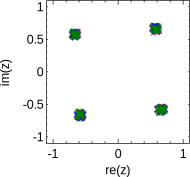
\includegraphics[width=\textwidth]{figures/matlab/res_450_qam4_cp_corr_pcorr}
    \caption{\gls{QAM}-4}
    \label{fig:res_450_qam4_cp_corr_pcorr}
  \end{subfigure}
  ~
  \begin{subfigure}{0.45\textwidth}
    \centering
    \includegraphics[width=\textwidth]{figures/matlab/res_450_qam256_cp_corr_pcorr}
    \caption{\gls{QAM}-256}
    \label{fig:res_450_qam256_cp_corr_pcorr}
  \end{subfigure}
  \caption{One Realization of Data received by the Narrow Band
    Transmission Setup after Channel and Phase Noise Correction}
  \label{fig:res_450_cp_corr_pcorr}
\end{figure}

\begin{figure}[p]
  \centering
  \begin{subfigure}{0.45\textwidth}
    \centering
    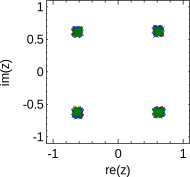
\includegraphics[width=\textwidth]{figures/matlab/res_450_qam4_cp_corr_pcorr_initial}
    \caption{\gls{QAM}-4}
    \label{fig:res_450_qam4_cp_corr_pcorr_initial}
  \end{subfigure}
  ~
  \begin{subfigure}{0.45\textwidth}
    \centering
    \includegraphics[width=\textwidth]{figures/matlab/res_450_qam256_cp_corr_pcorr_initial}
    \caption{\gls{QAM}-256}
    \label{fig:res_450_qam256_cp_corr_pcorr_initial}
  \end{subfigure}
  \caption{One Realization of Data received by the Narrow Band
    Transmission Setup after Channel, Initial Phase Rotation
    and Phase Noise Correction}
  \label{fig:res_450_cp_corr_pcorr_initial}
\end{figure}

\begin{figure}[p]
  \centering
  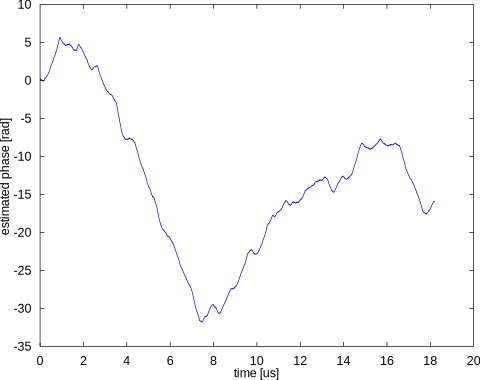
\includegraphics[width=0.8\textwidth]{figures/matlab/res_450_qam4_phase_est}
  \caption{One Realization of Phase Estimations vs. Time
    received by the Narrow Band Transmission Setup using \gls{QAM}-4}
  \label{fig:res_450_qam4_phase_est}
\end{figure}

\begin{figure}[p]
  \centering
  \begin{subfigure}{0.45\textwidth}
    \centering
    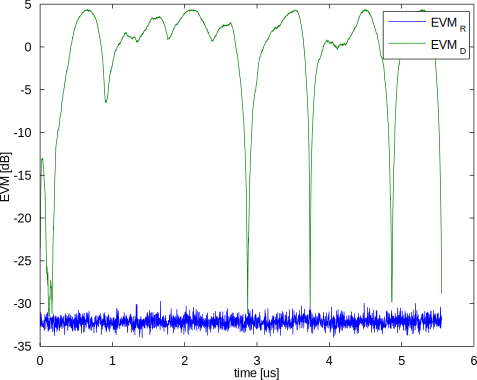
\includegraphics[width=\textwidth]{figures/matlab/res_450_qam4_evm}
    \caption{Before Phase Correction}
    \label{fig:res_450_qam4_evm}
  \end{subfigure}
  ~
  \begin{subfigure}{0.45\textwidth}
    \centering
    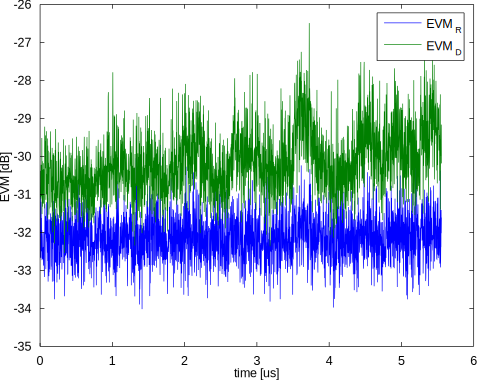
\includegraphics[width=\textwidth]{figures/matlab/res_450_qam4_evm_pcorr_initial}
    \caption{After Initial Phase and Phase Noise Correction}
    \label{fig:res_450_qam4_evm_pcorr_initial}
  \end{subfigure}
  \caption{One Realization of \gls{DEVM} and \gls{REVM}
    received by the Narrow Band Transmission Setup}
  \label{fig:res_450_qam4_evm_comparison}
\end{figure}

\chapter{Full Bandwidth Transmission}
\label{chap:res_1350}

To achieve even higher throughput than the one reached using 450 MS/s with \gls{QAM}-8,
higher symbols rates were analyzed using the exact same hardware as described
in \secref{sec:res_450_setup} and drawn in \figref{fig:res_450_bd}. Only a
few software parameters had to be changed. \\

The main difference of having a higher symbol rate is, that the signal does not
fit into a single Nyquist-zone anymore. Therefor the performance of the
quadrature baseband sampling gets important. \\

Using the exact same setup as in \chapref{chap:res_450} but with a symbol rate
of 1.8 GS/s a \gls{DEVM} of -7.73 was measured, which is significantly
worse than the in the 450 MS/s case. \\

\subsubsection{Simple Approach}
In order to investigate the cause of this sudden degradation of the \gls{DEVM},
we again look at a signal with 450 MS/s with an \gls{RX} \gls{IF}
of 2.2 GHz. When this signal is sampled at 1.8 GHz, we get the two signals
Re(Rx.Rf) and Im(Rx.Rf) shown in \figref{fig:res_450_freq_uncorr}.
After calculating the analytic signal shown in the second subplot,
we see that the negative frequency part does not fully cancel out
as it does in the simple theoretical model. \\

In order to improve the \acrfull{DEVM}, two correction coefficients, $\alpha$ and
$\beta$ were introduced which are applied on the second \gls{ADC} channel
before combining both channels to one complex signal \eqref{eq:res_1350_a_hat}.
$\alpha$ allows to correct time and $\beta$ phase differences between
the two channels. \\

\begin{figure}[p]
  \centering
  \begin{subfigure}{\textwidth}
    \centering
    \includegraphics[width=\textwidth]{figures/matlab/res_450_freq_uncorr_tx_rf}
    \caption{Transmitted \gls{IF} Signal}
    \label{fig:res_450_freq_uncorr_tx_rf}
  \end{subfigure}
  \vspace{4ex} \\
  \begin{subfigure}{\textwidth}
    \centering
    \includegraphics[width=\textwidth]{figures/matlab/res_450_freq_uncorr_rx_rf}
    \caption{Received \gls{IF} Signal after Sampling}
    \label{fig:res_450_freq_uncorr_rx_rf}
  \end{subfigure}
  \vspace{4ex} \\
  \begin{subfigure}{\textwidth}
    \centering
    \includegraphics[width=\textwidth]{figures/matlab/res_450_freq_uncorr_rx_rf_sup}
    \caption{Received \gls{IF} Signal $Re(Rx.Rf) + j \cdot Im(Rx.Rf)$}
    \label{fig:res_450_freq_uncorr_rx_rf_sup}
  \end{subfigure}
  \vspace{4ex} \\
  \begin{subfigure}{\textwidth}
    \centering
    \includegraphics[width=\textwidth]{figures/matlab/res_450_freq_uncorr_rx_usb}
    \caption{Received \gls{USBand} Signal}
    \label{fig:res_450_freq_uncorr_rx_usb}
  \end{subfigure}
  \vspace{4ex} \\
  \begin{subfigure}{\textwidth}
    \centering
    \includegraphics[width=\textwidth]{figures/matlab/res_450_freq_uncorr_rx_lsb}
    \caption{Received \gls{LSBand} Signal}
    \label{fig:res_450_freq_uncorr_rx_lsb}
  \end{subfigure}
  \caption{Spectrum Plots of Narrow Band Signal without any Correction}
  \label{fig:res_450_freq_uncorr}
\end{figure}

\begin{align}
  c[k] &= b[k] + j \cdot \hat a[k] \\
  \hat a[k] &= a[k]  \cdot \exp\left(
  \frac{-j}{2 \pi} \cdot \left(\frac{\alpha \cdot k}{N} + \beta\right)
  \right) \;\forall\; k \in \{0, 1, \dots,  N-1\}
  \label{eq:res_1350_a_hat}
\end{align}

To find the optimal correction coefficients, a coarse sweep was done to approximately
find the correct values followed by a more fine grained sweep over both parameters
which is shown in \figref{fig:res_1350_ab_sweep}.
The absolute minimum is reached for $\alpha = -0.08$ and $\beta = 0.096$. \\

Applying this correction to the 1.8 GS/s signal resulted in a significant
improvement of the \gls{DEVM} to -16.04 dB.

\begin{figure}[p]
  \centering
  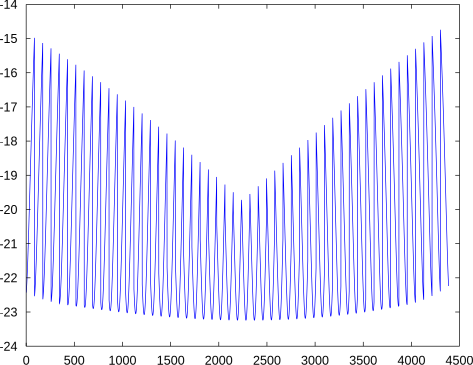
\includegraphics[width=0.8\textwidth]{figures/matlab/res_1350_ab_sweep}
  \caption{\gls{RDR} [dB] when sweeping over $\beta \in [0.07 \; 0.12]$
    (outer loop) and $\alpha \in [-0.17 \; 0.0]$ (inner loop)}
  \label{fig:res_1350_ab_sweep}
\end{figure}

\subsubsection{Signal Theory Approach}
Since the above approach requires a search over the optimal correction values,
a better approach was needed. Again in the case of the 450 MS/s signal,
the positive frequency half contains the desired signal and the negative frequency
half is supposed to be zero if the quadrature sampling would work as described
in the theory \secref{sec:rx_adc_1}. The real signal shows however an error
signal term in the negative frequency half which is assumed to be the
complex conjugate of the positive frequency half. By mirroring the desired signal
and correlating it with the error signal, one can see a strong
correlation peak showing that the error term is more or less the
desired signal attenuated by 10 dB and rotated by a fixed phase.
A corrected signal can be calculated by taking the signal, multiplying
it by this measured constant and subtracting this correction term
from the signal. This also works for the 1.8 GS/s case, where the desired
and the error signal fully overlap, because the error in the correction signal
due to the overlapping error signal is again another 10 dB attenuated.

\begin{align}
  s_{\text{sig}}[k] &= (s[k] + j \mathcal{H}\{s\}[k])/2 \\
  s_{\text{err}}[k] &= (s[k] - j \mathcal{H}\{s\}[k])/2 \\
  s_{\text{sig, mirr}}[k] &= s_{\text{sig}}^*[k] \\
  c[m] &= \sum_k s_{\text{sig, mirr}}[k+m] \cdot s_{\text{Err}}[k] \\
  C &= \frac{\sup_m c[m]}{\sum_k |s_{\text{sig}}[k]|^2} \\
  s_{\text{corr}}[k] &= s[k] - (s^*[k] .* C^*)
\end{align}

Using this correction approach, a \gls{DEVM} of -17.42 dB was achieved.

%%  LocalWords:  multi QAM Coupler coupler EVM Nyquist rx bd Matlab
%%  LocalWords:  AWG FPGA cnf BPSK FES CES PES awg ns DAC osci FFT eq
%%  LocalWords:  dBm pwr sivers BHP LSBand USBand WB Balun balun qam
%%  LocalWords:  Golay DEVM devm REVM affine ph ISI cp sys ces pcorr
%%  LocalWords:  pes evm baseband Im uncorr RDR adc sig mirr
